%!TEX root=../main.tex % Optional

\section{Einführung}

Diese Übung soll die Funktionsweise und Implementierung von eine Message Oriented Middleware (MOM) mit Hilfe des Frameworks Apache Active MQ demonstrieren. Message Oriented Middleware (MOM) ist neben InterProcessCommunication (IPC), Remote Objects (RMI) und Remote Procedure Call (RPC) eine weitere Moeglichkeit um eine Kommunikation zwischen mehreren Rechnern umzusetzen.

Die Umsetzung basiert auf einem praxisnahen Beispiel einer Windkraftanalage. Ein Windkraftanalage (Windrad) ist immer Teil eines Verbunds, genannt Windpark. Jede Windkraftanlage beinhaltet einen Rechner, der die Daten der Windkraftanalage aufzeichnet und diese steuern kann. Die Daten werden in einer XML-Struktur abgespeichert. Die Daten aller Windkraftanlagen eines Windparks werden von einem Parkrechner gesammelt und abgespeichert. Der Parkrechner kommuniziert mit einem Rechner der Zentrale. Eine Zentrale kommuniziert mit mehreren Windparks und steuert diese.

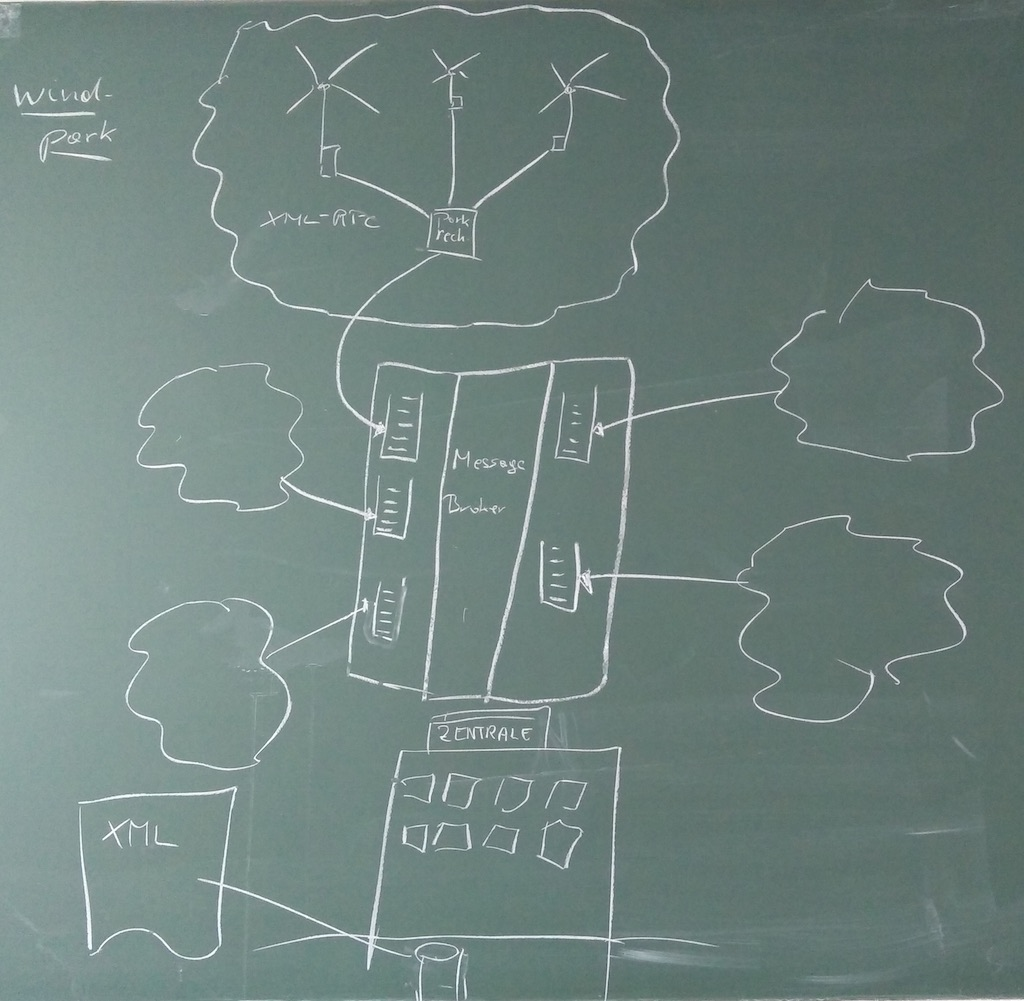
\includegraphics[scale=0.4]{images/windpark_grafik.jpg}

\subsection{Ziele}

Das Ziel dieser Übung ist die Implementierung einer Kommunikationsplattform von mehreren Windparks mit einer zentralen Stelle unter Verwendung einer Message Oriented Middleware (MOM). Hier sollen nun die Parkrechner von mehreren Windparks die gesammelten Daten an eine zentrale Stelle übertragen. Aufgrund der Offenheit von nachrichtenbasierten Protokollen werden hier Message Queues verwendet. So kann gewährleistet werden, dass in Zukunft weitere Anlagen hinzugefügt bzw. Kooperationspartner eingebunden werden können.

\subsection{Voraussetzungen}

\begin{itemize}
    \item Grundlagen Architektur von verteilten Systemen
    \item Grundlagen zur nachrichtenbasierten Systemen / Message Oriented Middleware
    \item Verwendung des Message Brokers Apache ActiveMQ
    \item Verwendung der XML-Datenstruktur eines Parkrechner "parknodedata.xml"
    \item Verwendung der JMSChat.jar JAVA Applikation als Startpunkt für diese Aufgabenstellung
\end{itemize}

\subsection{Aufgabenstellung}

Implementieren Sie die Windpark-Kommunikationsplattform mit Hilfe des Java Message Service. Verwenden Sie Apache ActiveMQ (http://activemq.apache.org) als Message Broker Ihrer Applikation. Das Programm soll folgende Funktionen beinhalten:

\begin{itemize}
    \item Jeder Windpark (Parkrechner) erstellt eine Message Queue mit einem vorgegeben Namen.
    \item Der Parkrechner stellt die gesammelten Daten der Windkraftanlagen diese Message Queue.
    \item Der Zentralrechner lädt aus einer Konfigurationsdatei die Namen (Message Queues) aller Parkrechner.
    \item Der Zentralrechner verbindet sich mit allen Message Queues und empfängt die Daten der Windparks.
    \item Der Zentralrechner sammelt die Daten der Windparks und legt diese erneut in einer XML-Datei ab. Hier wird die XML-Struktur dynamisch erweitert, indem in der XML-Struktur der Name des Parkrechners und die Übertragungszeit abgelegt werden.
    \item Bei erfolgreicher Übertragung der Daten wird dem Parkrechner die Nachricht ''SUCCESS'' übertragen. Die Umsetzung der Rückmeldung ist vom Software-Entwickler zu entwerfen und umzusetzen.
\end{itemize}

Die Applikation ist über das Netzwerk mit anderen Rechnern zu testen!

\subsection{Bewertung}

\begin{itemize}
    \item Gruppengrösse: 1 Person
    \item Anforderungen ''überwiegend erfüllt''
    \begin{itemize}
        \item Implementierung der Kommunikation zwischen einem Parkrechner und dem Zentralrechner (JMS Queue)
    \end{itemize}
    \item Anforderungen ''zur Gänze erfüllt''
    \begin{itemize}
        \item Implementierung der Kommunikation mit mehreren Parkrechner und dem Zentralrechner
        \item Rückmeldung des Ergebnisses der Übertragung vom Zentralrechner an die Parkrechner (JMS: Topic)
        \item Zusammensetzung der Daten aller Windparks in eine zentrale XML-Struktur
    \end{itemize}
\end{itemize}

\subsection{Fragestellung für Protokoll}

\begin{itemize}
    \item Nennen Sie mindestens 4 Eigenschaften der Message Oriented Middleware?
    \item Was versteht man

Richard Wutscher, [26.04.18 14:10]
unter einer transienten und synchronen Kommunikation?
    \item Beschreiben Sie die Funktionsweise einer JMS Queue?
    \item JMS Overview - Beschreiben Sie die wichtigsten JMS Klassen und deren Zusammenhang?
    \item Beschreiben Sie die Funktionsweise eines JMS Topic?
    \item Was versteht man unter einem lose gekoppelten verteilten System? Nennen Sie ein Beispiel dazu. Warum spricht man hier von lose?
\end{itemize}

\subsubsection{Links \& Dokumente}

\begin{itemize}
    \item Grundlagen Message Oriented Middleware: Praesentation
        \item XML-Datenstruktur eines Parkrechner: parknodedata.xml
        \item Middleware: Apache ActiveMQ Installationspaket
        \item Beispiel Quellcode: JMSChat.jar
        \item Apache ActiveMQ \& JMS Tutorial:

    \begin{itemize}
        \item http://activemq.apache.org/index.html
        \item http://www.academictutorials.com/jms/jms-introduction.asp
        \item http://docs.oracle.com/javaee/1.4/tutorial/doc/JMS.html\#wp84181
        \item http://www.onjava.com/pub/a/onjava/excerpt/jms\_ch2/index.html
        \item http://www.oracle.com/technetwork/systems/middleware/jms-basics-jsp-135286.html
        \item http://www.oracle.com/technetwork/articles/java/introjms-1577110.html
    \end{itemize}
\end{itemize}

